%!TEX root=../document.tex

\section{Quantenkryptographie}
\label{sec:Quantenkryptographie}

\subsection{One-Time-Pad}

Das One-Time-Pad ein symmetrisches Verschlüsselungsverfahren und funktioniert über einen Schlüssel welcher folgende Eigenschaften erfüllen muss: \cite{onetimepadwiki}
\begin{itemize}
    \item er ist mindestens so lang wie die Nachricht
    \item er ist gleichverteilt zufällig gewählt
    \item er muss geheim bleiben
    \item er darf nicht wiederverwendet werden, auch nicht teilweise
\end{itemize}

Damit erfüllt ein One-Time-Pad Kerckhoffs’ Prinzip, welches besagt, dass die Sicherheit eines Kryptosystems nicht von der Geheimhaltung des Verschlüsselungsalgorithmus abhängen darf, sondern lediglich von der Geheimhaltung des Schlüssels.\cite{onetimepadwiki}

Es erfüllt daher folgende Kriterien:

\begin{itemize}
    \item Es gibt genauso viele Schlüssel wie mögliche Chiffate
    \item Zu jedem Klartext-Chiffrat-Paar gibt es genau einen Schlüssel, der auf den Klartext angewendet das Chiffrat ergibt
\end{itemize}

Dies bedeuted, dass eine mit einem One-Time-Pad Verschlüsselte Nachricht auch mit beliebig hoher Rechenleistung nicht entschlüsselt werden kann, \cite{cryptintroduction} da auch statistische Methoden, welche bei anderen Verschlüsselungsmethoden dazu verwendet werden können, um die Nachricht zu dechiffrieren, bei einem One-Time-Pad nicht funktionieren.

Beim One-Time-Pad handelt es sich also quasi um ein 'perfektes' Verschlüsselungssystem. 
Das größte Problem des One-Time-Pads ist es allerdings, den geheimen Schlüssel an beide Parteien zu übertragen, ohne, dass dieser abgefangen wird.


\subsection{Quanten-Schlüsselaustausch}
\label{sec:Quanten-Schlusselaustausch}

Als Quanten-Schlüsselaustausch bezeichnet man Verfahren der Quanteninformatik, die Eigenschaften der Quantenmechanik nutzen, um zwei Parteien eine gemeinsame Zufallszahl zur Verfügung zu stellen.
Dies löst nun das größte Problem des One-Time-Pad, nämlich die sichere Übertragung des Schlüssels.
Der Quanten-Schlüsselaustausch hat grundlegend nichts mit Quantencomputern zu tun und benötigt auch keinen um durchgeführt zu werden.
Erste Theorien wurden bereits 1984 aufgestellt und 2004 ein erster Banktransfer über einen durch einen Quanten-Schlüsselaustausch erstellten Schlüssel getätigt. \cite{experiement_qsa}

Der Quanten-Schlüsselaustausch funktioniert durch das ''No-Cloning-Theorem'' nach dem Prinzip, einen Angreifer (Man in the Middle) bei der Schlüsselgenerierung zu erkennen, da eine Messung eines quantenmechanischen Zustandes, immer den Wert verändert.


\subsubsection{Funktionsweise}

Die Informationen werden mittels Photonen übertragen. Photonen können horizontal oder vertikal polarisiert sein (– oder |). Ein horizontal polarisiertes Photon wird von einem vertikalen Filter reflektiert, durch einen horizontalen durchgelassen.
Außerdem können Photonen verschiedenartig diagonal polarisiert sein (/, ''rechtsdiagonal'', oder \textbackslash, ''linksdiagonal''). Diese werden wieder von ihren respektiven Filtern reflektiert, oder durchgelassen.
Daraus ergeben sich nun 2 Basen, die +-Basis (- und |) und die $\times$-Basis (/ und \textbackslash).
Jede Polarisation einer Basis bekommt nun einen anderen binären Wert zugewiesen, wobei die Wahl dabei irrelevant ist, sie muss nur bei beiden Parteien gleich sein. 

\begin{figure}[!htb]
	\centering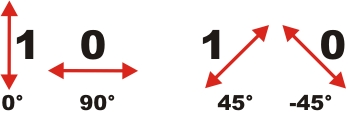
\includegraphics[width=0.6\textwidth]{images/polarisation}
	\caption{Messbasis + (links) und Messbasis $\times$ (rechts) \cite{quantenschluesselaustausch}}
	\label{fig:polarisation}
\end{figure}

Nun beginnt der Sender der Nachricht (Alice), einzelne Photonen an den Empfänger (Bob) zu verschicken. Beide wählen dabei komplett zufällig, mit gleich großer Wahrscheinlichkeit eine Basis aus. 
Alice wählt nun weiters, wieder komplett zufällig und gleichverteilt eine Polarisation aus der ausgewählten Basis und sendet so ein Photon an Bob.

Bob wählt nun auch komplett zufällig und gleichverteilt eine Messbasis aus.
Wenn Bob nun zufällig die gleiche Basis wie Alice verwendet hat, bekommt dieser ein gültiges Ergebnis (also 0 oder 1), wenn er allerdings eine andere Basis verwendet hat wird das gesendete Photon zu 50\% reflektiert oder durchgelassen, ergibt also zu 50\% 0 oder 1, diese Messung ist nicht brauchbar und wird später verworfen.

Nachdem Alice genügend Photonen an Bob geschickt hat, müssen beide Parteien noch bestimmen, welche Messwerte für den Schlüssel verwendet werden sollen.
Dafür machen Alice und Bob die Wahl ihrer Messbasis öffentlich, jedoch nicht welche Polarisation gesendet bzw. empfangen wurde. Sie veröffentlichen also beide eine Liste mit denen von ihnen gewählten Basen (+ oder $\times$).
Schlussendlich vergleichen beide nun diese Listen, wenn sie bei einer Übertragung die gleiche Basis verwendet haben wird der Wert für den Schlüssel verwendet, ansonsten einfach verworfen.
Dadurch werden also ungefähr 50\% der gesendeten bits für die Schlüsselgenerierung verwendet.

\newpage

\begin{table}[ht]
    \centering
    \setlength\tabcolsep{4pt}
    \begin{minipage}{.45\textwidth}
        \centering
        \begin{tabular}{|c|c|c|}
        \hline
        Photon      & Basis     & Bit           \\ \hline
        \textbf{1}  & +         & \textbf{1}    \\ \hline
        2           & $\times$  & 1             \\ \hline 
        \textbf{3}  & +         & \textbf{0}    \\ \hline
        4           & +         & 1             \\ \hline
        \textbf{5}  & $\times$  & \textbf{1}    \\ \hline
        \textbf{6}  & +         & \textbf{0}    \\ \hline
        \textbf{7}  & $\times$  & \textbf{0}    \\ \hline
        8           & $\times$  & 1             \\ \hline
        \end{tabular}
        \caption{Beispielübertragung Alice}
    \end{minipage}%
    \hfill
    \begin{minipage}{.45\textwidth}
        \centering
        \begin{tabular}{|c|c|c|}
        \hline
        Photon      & Basis     & Bit           \\ \hline
        \textbf{1}  & +         & \textbf{1}    \\ \hline
        2           & +         & 0             \\ \hline 
        \textbf{3}  & +         & \textbf{0}    \\ \hline
        4           & $\times$  & 1             \\ \hline
        \textbf{5}  & $\times$  & \textbf{1}    \\ \hline
        \textbf{6}  & +         & \textbf{0}    \\ \hline
        \textbf{7}  & $\times$  & \textbf{0}    \\ \hline
        8           & +         & 0             \\ \hline
        \end{tabular}
        \caption{Beispielmessungen Bob}
    \end{minipage}
\end{table}

In diesem Beispiel sind die \textbf{Fett} hervorgehoben Basen gleich, also wäre der generiert Schlüssel von Alice und Bob 10100; jeweils Photon 1, 3, 5, 6, 7 werden verwendet, die anderen werden verworfen.


\subsubsection{Abhörsicherheit}

Bei dem obigen Verfahren ist es nun auch möglich Abhörsicherheit zu garantieren, sodass eine dritte Person (Eve) sich nich zwischen die Kommunikation schalten und den Schlüsselaustausch abfangen kann.

Um zu versuchen die Kommunikation abzufangen kann Eve sich zwischen Bob und Alice schalten.
Allerdings muss Eve, genauso wie Bob zuerst das gesendete Photon messen und wählt dafür eine zufällige Basis.
Eve muss allerdings sofort wieder ein neues Photon an Bob senden, in 50\% der Fälle wählt Eve zur Messung jedoch die falsche Basis und sendet dadurch ein falsches bit an Bob.
Diesen durch Eve verursachten Fehler können Alice und Bob nun bemerken, wenn sie die gleiche Basis gewählt haben, da sie bei gleicher Wahl immer eindeutige Ergebnisse erhalten sollten.
Außerdem kann Eve so nie den kompletten Schlüssel bekommen, da sie das bit an einer Stelle bei der sie eine falsche Basis verwendet hat, nicht herausfinden kann.

\begin{table}[ht]
    \centering
    \begin{tabular}{|c|c|c|c|c|}
    \hline
    Basis Alice/Bob     & Basis Eve & Empfang Bob   & Übereinstimmung Alice und Bob \\ \hline
    +~+                 & +         & Eindeutig     & 100\% \\ \hline
    +~+                 & $\times$  & Zufall        & 50\%  \\ \hline 
    $\times$~$\times$   & +         & Eindeutig     & 50\%  \\ \hline
    $\times$~$\times$   & $\times$  & Zufall        & 100\% \\ \hline
    
    \end{tabular}
    \caption{Möglichkeiten der Übertragung mit Eve als Man-in-the-Middle \cite{quantenschluesselaustausch}}
    \label{table:eve-moeglichkeiten}
\end{table}

Insgesamt gibt es, wenn Alice und Bob die gleiche Basis gewählt haben, in 25\% der Fällen falsche Messergebnisse. 
Um Eve also zu entdecken müssen Bob und Alice nach der erfolgreichen Übertragung einen Abgleich von einigen (nicht allen!) Werten, bei denen sie die gleiche Basis verwendet haben durchführen, gibt es dort über 25\% Diskrepanz zwischen den Werten, ist sehr Wahrscheinlich ein Man-in-the-Middle Angriff durchgeführt worden.


\subsection{Post-Quanten-Kryptographie}
\label{sec:Post-Quanten-Kryptographie}

Ein besonderer Teil der Quantenkryptographie stellt die Post-Quanten-Kryptographie dar.
Diese behandelt sich mit der Tatsache, dass alle modernen asymmetrischen Verschlüsselungsverfahren durch die Entwicklung eines Quantencomputers unbrauchbar werden.

Die Sicherheit der momentanen Verschlüsselungsverfahren basiert auf den 3 komplizierten mathematischen Problemen:

\begin{itemize}
    \item Faktorisierungsproblem
    \item Diskreter-Logarithmus Problem
    \item Elliptic Curve Cryptography Problem
\end{itemize}

Die obigen Probleme können durch einen Quantencomputer mit Shor's Algorithms innerhalb kürzester Zeit gelöst werden. (siehe \ref{sec:Shor's Algorithmus}).

Damit also momentane Kommunikation auch in Zukunft nicht entschlüsselt werden kann, benötigt man auch jetzt schon Verschlüsselungsverfahren, welche auch Quantencomputer nicht knacken können. \cite{postquantumwiki}


\subsubsection{Post-Quanten-Verschlüsselungsalgorithmen}
\label{sec:Post-Quanten-Verschluesselungsalgorithmen}

Die aktuelle Post-Quanten-Kryptographie Forschung fokussiert sich auf 6 Bereiche: \cite{postquantumwiki}

\begin{itemize}
    \item \textbf{Lattice-based cryptography}
    \item \textbf{Multivariate cryptography}
    \item \textbf{Hash-based cryptography}
    \item \textbf{Code-based cryptography}
    \item \textbf{Supersingular elliptic curve isogeny cryptography}
    \item \textbf{Symmetric key quantum resistance}
\end{itemize}


\subsubsection{Symmetrische Schlüssel Resistenz}
\label{Symmetrische Schlüssel Resistenz}

Symmetrische Schlüssel mit ausreichender Länge, sind bereits heute immun gegen Angriffe von Quantencomputern. \cite{symkeyresistance} 
Zwar können Quantencomputer auch effektivere Brute-Force Angriffe auf einen symmetrischen Schlüssel durchführen, allerdings wird dieser nicht exponentiell schneller, wie bei der asymmetrischen Verschlüsselung.
Darum reicht es einfach, die Schlüssellange zu erhöhen.

\newpage


\section{Quantenalgorithmik}
\label{sec:Quantenalgorithmik}


\subsection{Besonderheiten und Unterschiede zu ''klassischer'' Algorithmik}
\label{sec:Besonderheiten und Unterschiede zu klassischer Algorithmik}

Ein ''klassischer'' (nicht quanten) Algorithmus ist eine endliche Sequenz von Maschineninstruktionen, wo jede Instruktion auf einem klassischen Computer ausgeführt wird.
Ähnlich sind Quantenalgorithmen eine endliche Sequenz von Quanteninstruktionen, welche auf einem Quantencomputer ausgeführt werden. Jedoch kann ein Quantencomputer auch klassische Algorithmen ausführen. \cite{quantenalgorithmgwiki}

Die Besonderheiten von Quantenalgorithmen liegen in der Verwendung von Qubits (siehe \ref{sec:Qubit}), welche quantenmechnische Prinzipien wie die Quantenteleportation und die Superposition verwenden.
Zwar gibt es bereits einige entwickelte Quantenalgorithmen, allerdings ist dieses Gebiet noch nicht sehr gut erforscht.


\subsection{Quantenalgorithmik Übersicht}
\label{sec:Quantenalgorithmik Übersicht}


\subsubsection{Deutsch-Josza Algorithmus}

Dieser Algorithmus kann zum Lösen sogenannter Blackbox-Probleme verwendet werden, für die normale Computer exponentiell viele Zugriffe, ein Quantencomputer allerdings nur einen bräuchte.
Hierbei wird z.B. das Ergebnis einer Funktion $f$ darauf überprüft, ob alle Eingaben konstant 0 als Ergebnis liefern, oder ob beispielsweise die eine Hälfte 0 und die andere Hälfte 1 liefert. \cite{quantenalgorithmgwiki}


\subsubsection{Simons's Algorithmus}

Dieser Algorithmus dient auch zur exponentiell schnelleren Lösung von Blackbox-Problemen und war Vorbild für Shor's Algorithmus. \cite{quantenalgorithmgwiki}

\subsubsection{Quanten Phasen Näherungs-Algorithmus}

Aus der englischen Wikipedia:\cite{quantenalgorithmgwiki}
\begin{quote}
    \textit{The quantum phase estimation algorithm is used to determine the eigenphase of an eigenvector of a unitary gate given a quantum state proportional to the eigenvector and access to the gate.}
\end{quote}
Der Algorithmus wird außerdem oft als Unterfunktion in anderen Quantenalgorithmen verwendet. 


\subsection{Shor's Algorithmus}
\label{sec:Shor's Algorithmus}

Shor's Algorithmus ist ein Quantenmechanischer Algorithmus aus dem mathematischen Gebiet der Zahlentheorie.
Er dient dabei zur Ermittlung eines nicht trivialen Teilers und zählt damit zu den Faktorisierungsalgorithmen.
Für die Faktorisierung einer Zahl $n$ benötigt ein Quantencomputer mindestens $\log{n}$ Qubits.

\newpage

Shor's Algorithmus hat folgende Eigenschaften: \cite{shorwiki}

\begin{itemize}
    \item Eingabe:  zusammengesetzte Zahl $n$
    \item Ausgabe:  ein nicht trivialer Faktor von $n$
    \item Laufzeit: $O((\log{n})^3)$ Gatteroperationen 
\end{itemize}

Shor's Algorithmus läuft also in polynomieller Zeit und ist dem besten bis jetzt bekannten klassischen Faktorisierungsalgorithmus, dem Zahlkörpersieb, welches mit sub-exponentieller Zeit läuft weit überlegen.
Der Zahlenkörpersieb Algorithmus hat eine ungefähre Laufzeit von $O(e^{1.9 (\log{N})^{1/3} (\log{\log{N}})^{2/3}})$. \cite{numberfieldsieve}


Shor's Algorithmus kann man Grundlegend in 2 Teile teilen: einen Klassischen- und einen Quantenteil.
Der Klassische Teil wird zur Reduzierung des Problems verwendet, der Quantenteil dient dann zu effektiven Lösung des Restproblems.


\subsection{Grover's Algorithmus}
\label{sec:Grover's Algorithmus}

Grover's Algorithmus ist ein Quantenalgorithmus zur Suche in einer unsortierten Datenbank mit $N$ Einträgen. Er löst dabei das Problem mit $O(\sqrt{N})$ Schritten und $O(\log N)$ Speicherbedarf.

Die prinzipiell schnellstmögliche Suche in einer unsortierten Datenbank auf einem klassischen Computer, die Linearsuche benötigt dabei $O(N)$ Rechenschritte.
Durch Grover's Algorithmus ergibt sich eine beträchtliche quadratische Beschleunigung gegenüber der Linearsuche.


\subsection{Quanten Programmierung}
\label{sec:Quanten Programmierung}

Es gibt bereits einige Quantenprogrammierprachen, welche bereits zum Ausdruck von Quantenalgorithmen verwendet werden können.
Im Moment gibt es 2 Gruppen von Quantenprogrammiersprachen: Imperative und Funktionale.

Die 2 bekanntesten der ersten Gruppe sind QCL \cite{qcl} und LanQ \cite{lanq}.


\subsubsection{QCL - Quantum computing language}
\label{sec:QCL - Quantum computing language}

QCL ist eine Erweiterung von C; Die Syntax ist identisch mit der von C, mit einigen Quantenmechnanischen Erweiterungen.
Außerdem kann ''klassischer'' und quanten - Code in einem Programm zusammen verwendet werden.

Der grundlegendste quanten-Datentyp in QCL ist das qureg (Quanten Register).
Es ist quasi ein Array von qubits: \cite{quantenprogwiki}

\begin{lstlisting}
qureg x1[2]; // 2-qubit quantum register x1
qureg x2[2]; // 2-qubit quantum register x2
H(x1); // Hadamard operation on x1
H(x2[1]); // Hadamard operation on the first qubit of the register x2
\end{lstlisting}

\newpage

Außerdem kann, da die Quantenoperationen nur Simuliert werden, der Status des Programms abgerufen werden: \cite{quantenprogwiki}

\begin{lstlisting}
qcl> dump
: STATE: 4 / 32 qubits allocated, 28 / 32 qubits free
0.35355 |0> + 0.35355 |1> + 0.35355 |2> + 0.35355 |3>
+ 0.35355 |8> + 0.35355 |9> + 0.35355 |10> + 0.35355 |11>
\end{lstlisting}

Eine der wichtigsten Funktionen der Sprache ist die Möglichkeit Operationen und Funktionen zu definieren, mit denen Quanteninformation manipuliert werden können.
Zum Beispiel: \cite{quantenprogwiki}

\begin{lstlisting}
operator diffuse (qureg q) {
    H(q);                 // Hadamard Transform
    Not(q);               // Invert q
    CPhase(pi, q);        // Rotate if q=1111..
    !Not(q);              // undo inversion
    !H(q);                // undo Hadamard Transform
}
\end{lstlisting}
